\documentclass[11pt, a4paper]{article}
%\usepackage{proj1}
\usepackage{natbib}
\usepackage{fancyhdr}  
\usepackage{subcaption}
\usepackage{caption}
\usepackage{graphicx}
\usepackage{numprint}
\usepackage{multirow}
\linespread{1.25} 
\setlength{\parindent}{0cm}
\graphicspath{{Images/}}
\usepackage{hyperref}
\usepackage{amsmath}
\usepackage{amsfonts}
\usepackage{amssymb}
\usepackage{amsthm}
\usepackage{mathtools}
\usepackage{commath}
\usepackage{bbm}

%\usepackage[sc,osf]{mathpazo}
\usepackage{subcaption}
\usepackage[a4paper, top=1in, left=1.0in, right=1.0in, bottom=1in, includehead, includefoot]{geometry} %Usually have top as 1in

\usepackage{listings}
\usepackage{color} %red, green, blue, yellow, cyan, magenta, black, white
\definecolor{mygreen}{RGB}{28,172,0} % color values Red, Green, Blue
\definecolor{mylilas}{RGB}{170,55,241}


\hypersetup{colorlinks,linkcolor={black},citecolor={blue},urlcolor={black}}
\usepackage{color}
\urlstyle{same}


\theoremstyle{definition}
\newtheorem{definition}{Definition}[section]

%\newcommand{\Sta}{\rho}
\newcommand{\Adj}{p}
\newcommand{\adj}{q}
%\newcommand{\Con}{u}
\newcommand{\Sta}{\rho}
\newcommand{\Stav}{\mathbf{v}}
\newcommand{\Adja}{\mathbf{p}}
\newcommand{\Adjb}{q}
\newcommand{\Adjc}{{p}_{\partial \Sigma}}
\newcommand{\Con}{\mathbf{f}}
\newcommand{\nor}{\mathbf{n}}




\pagenumbering{gobble}
\begin{document}
	
\section{Update Scheme}
I haven't found anything useful in the literature yet. I have mainly found things involving gradient decent methods, or different kind of fixed point schemes (which may be worth looking into in general).
I have looked at a way of making the adaptive method dependent on the error rather than the iteration count, but haven't been that successful in finding good cutoffs.
I started looking at a method which increases $\lambda$ not in steps but by using the $\ln$ function. This seems to work well, see Figures \ref{F1}, \ref{F2}. I think there is again ways to improve this, either by trying different things, or by finding the right inspiration in the literature. 

\begin{figure}[h]
	\centering
	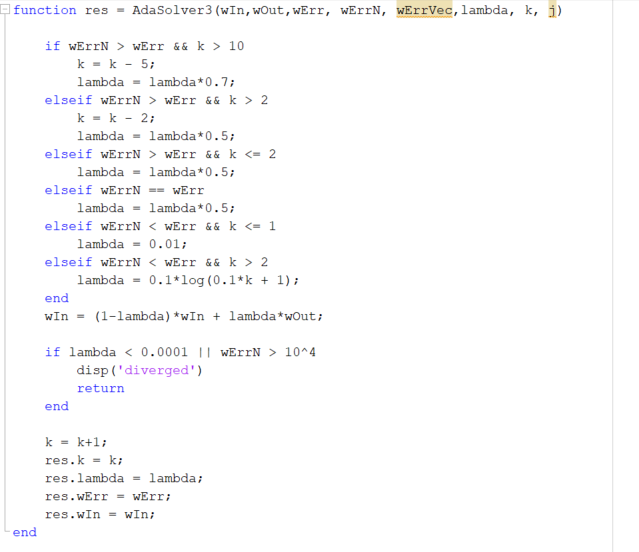
\includegraphics[scale=0.8]{Screen1.png}
	\caption{New Adaptive Method, $k$ starts at $1$, $wErrN$ is the error at this iteration, $wErr$ is at the previous iteration.} 
	\label{F1}
\end{figure}
\begin{figure}[h]
	\centering
	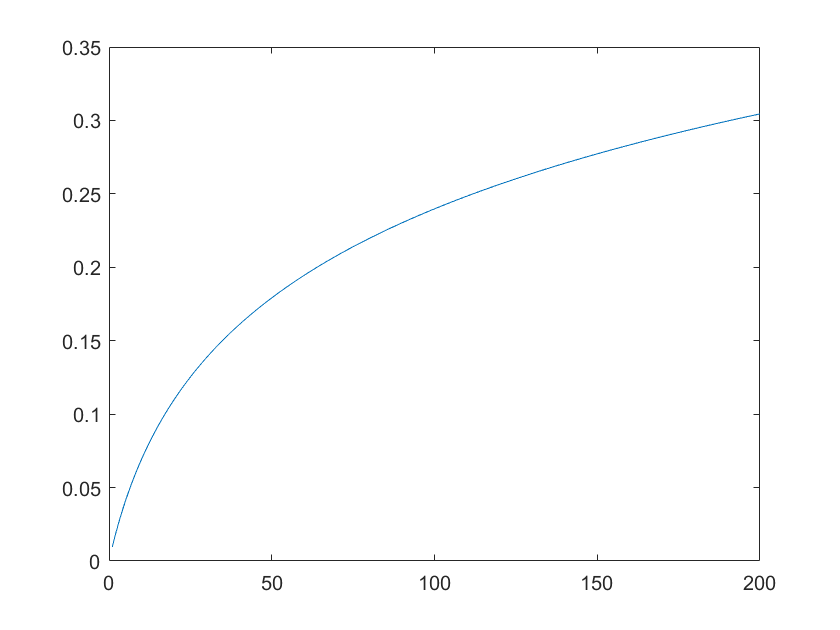
\includegraphics[scale=0.4]{Plot1.png}
	\caption{$\lambda$ vs iterations} 
	\label{F2}
\end{figure}

\subsection{Convergence}
The convergence plots are generally very similar and look like Figures \ref{F3}/ \ref{F4}. Maybe there is a case for adapting $\lambda$ to reflect the convergence pattern somehow? Because in the plot it looks like $\lambda$ drives the error down in the beginning, so that the tolerance is reached sooner, but doesn't change the shape of convergence.However, I am not sure if that is possible, given that the error is quite sensitive to $\lambda$ even when it's low and slowly changing.
\begin{figure}[h]
	\centering
	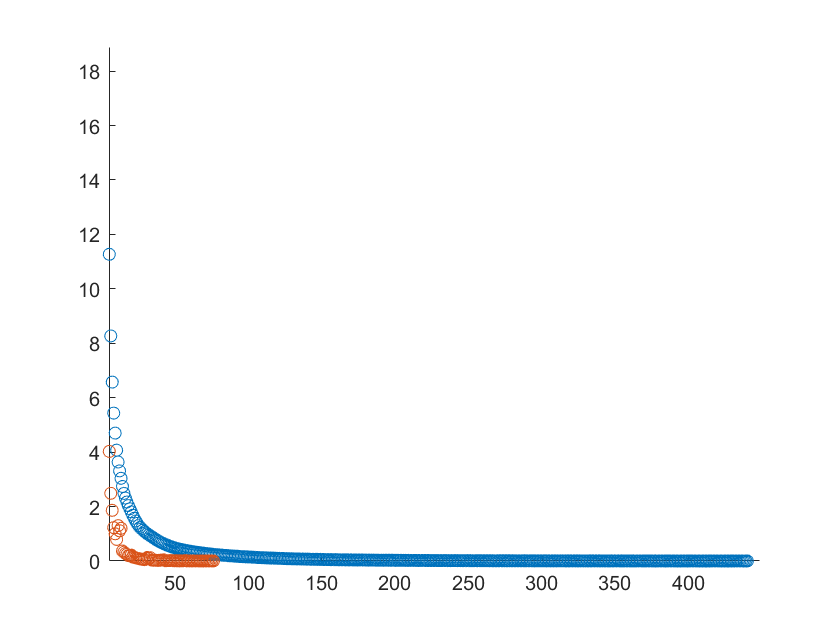
\includegraphics[scale=0.6]{Ex10a.png}
	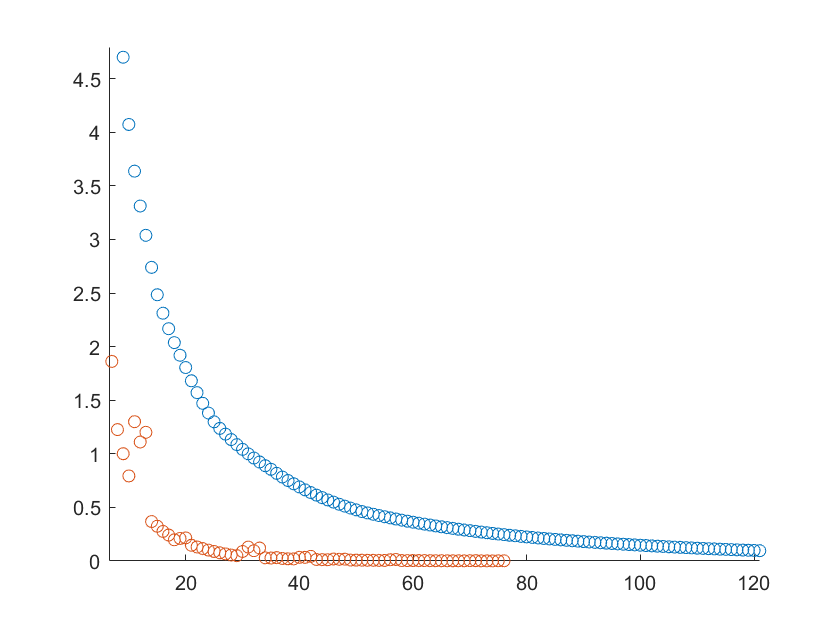
\includegraphics[scale=0.4]{Ex10b.png}
	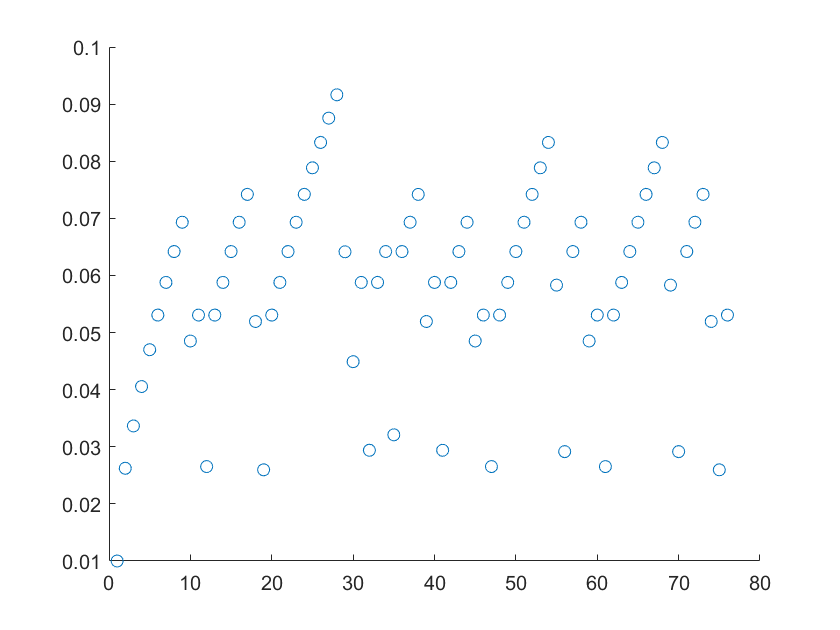
\includegraphics[scale=0.4]{lambdaVec10.png}
	\caption{Convergence Plots (blue is $\lambda$ constant, red is adaptive); change in $\lambda$ with iteration (figure 3)} 
	\label{F3}
\end{figure}
	
\begin{figure}[h]
	\centering
	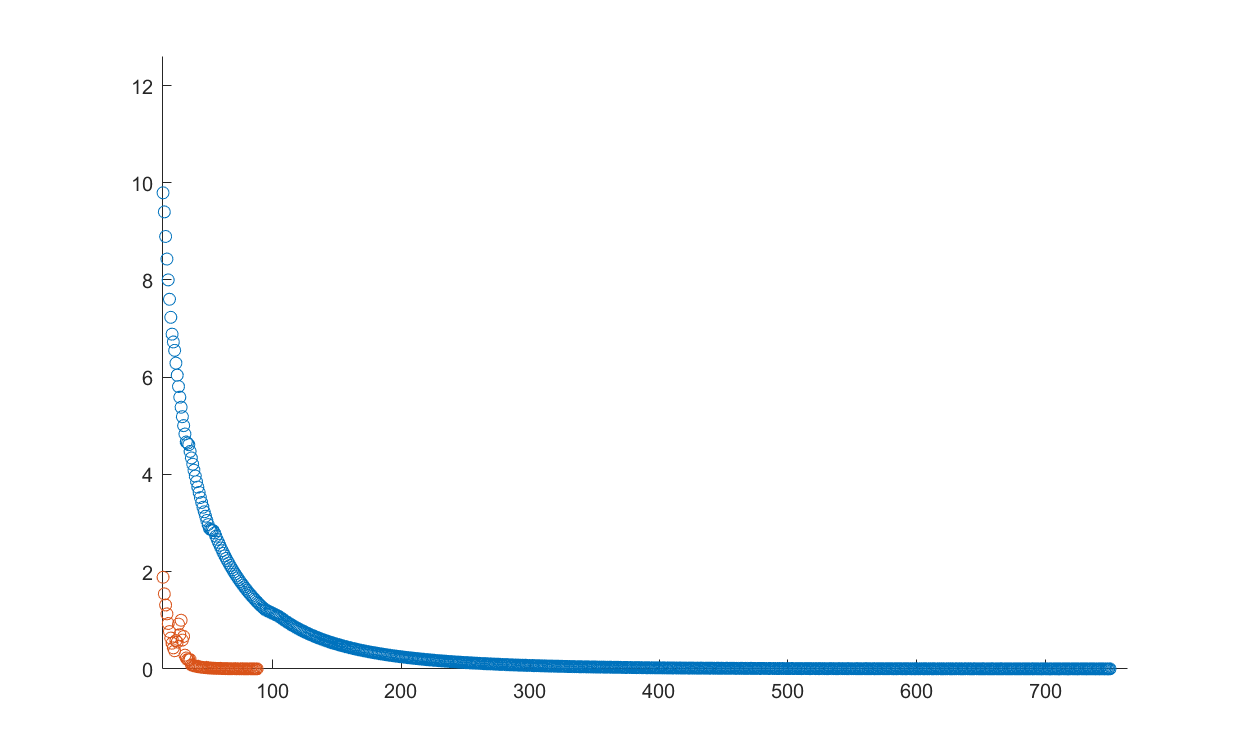
\includegraphics[scale=0.6]{Ex11.png}
	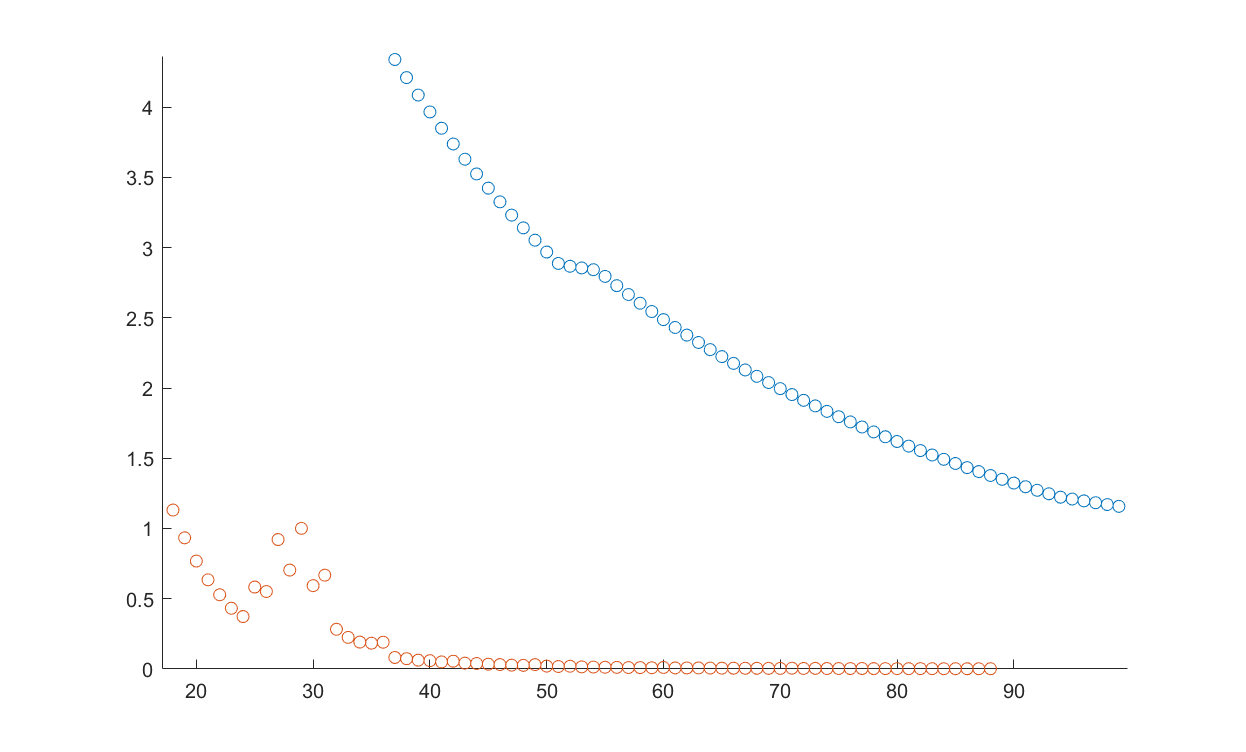
\includegraphics[scale=0.4]{Ex11a.png}
	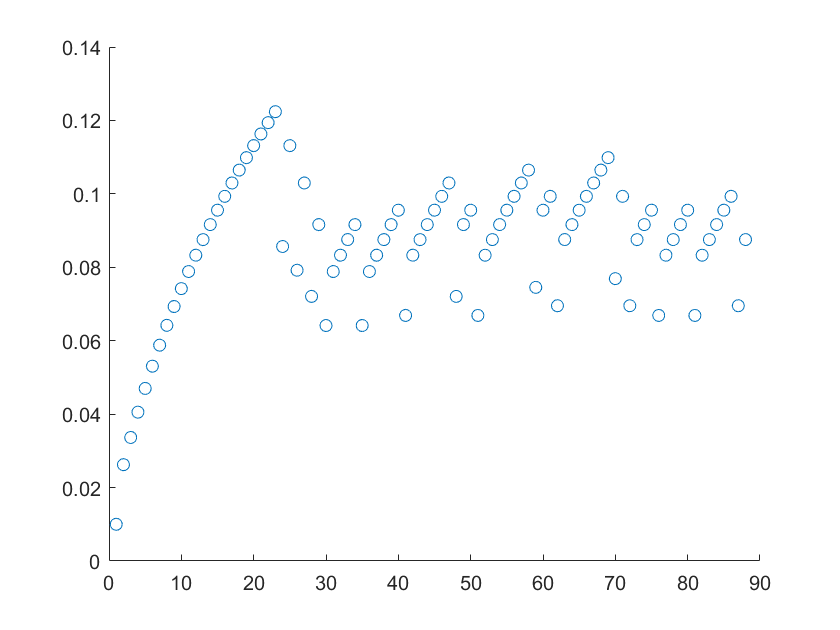
\includegraphics[scale=0.4]{lambdaVec11.png}
	\caption{Convergence Plots (blue is $\lambda$ constant, red is adaptive)change in $\lambda$ with iteration (figure 3)} 
	\label{F4}
\end{figure}	
	
\section{The in/outflow problem}
	I fixed a few mistakes in the code, however it is still not running as nicely. I haven't gotten around to doing everything we suggested trying last week.
	However, if I set the forward problem (with $w=0$) as the target, the problem converges within one iteration. I then tried a very small perturbation of this target (without changing the boundaries as we have done in the past). Choosing $\beta = 10^{-1}$, this problem converges to the set error tolerance of $10^{-3}$, however not for $\beta = 10^{-2}$.
	I think this shows that it is working in principle, but that these problems are generally hard. I tried targets further away from the forward problem, and I need to set $\lambda$ much smaller and it takes way too long to converge (if it does converge).
	Next I will go the step back to the constant flow on one boundary.

\section{Sparse to fine grid}
Using $10^{-7}$ ODE throughout.
Testing the exact problem and perturbing it works. There is some gain in iterations. Essentially the fine grid picks up where the sparse grid has left off (e.g. if I run the sparse grid up to a tolerance of $0.1$, then the fine grid starts at $0.1$ and continues). A time saving can be made because in the exact problem I can run the entire problem (up to the desired optimality tolerance) on the sparse grid. Then the fine grid converges in one iteration. This is faster because each iteration is faster on the sparse grid.
Example: For sparse grid choose $N =22$ and for fine $N = 40$. If we choose to run the sparse grid to an optimality tolerance of $1$, this converges within 1 iteration and $2$ seconds. We get an output error of $0.0388$, which is the same when we interpolate the solution onto the fine grid. It takes $285$ iterations and $4000$s to converge to an error of $2.8313 \times 10^{-4}$.\\
In comparison, letting the sparse grid run to the optimality tolerance of $10^{-3}$ (equal to the fine grid), we get that we converge in $357$ iterations and $655$ seconds. The output error (equal to the interpolated error) is $2.7060 \times 10^{-4}$. The fine grid takes one iteration to converge, which is $30$ seconds and the final error is $1.0792 \times 10^{-4}$. While the second option takes more iteration, it is quite a large saving of time.   

However, this does not translate one to one to non exact problems, but I am still in the process of working this out exactly. But the interpolation is not as exact I think because the error of the sparse grid is not equal to the initial error of the fine grid. 	
	
	
	
	
	
	
	
	
\end{document}